\chapter{LHC y detector ATLAS}
% \addcontentsline{toc}{chapter}{LHC y detector ATLAS}



\chaptermark{LHC y detector ATLAS}




El Gran Colisionador de Hadrones (\textit{\textbf{L}arge \textbf{H}adron \textbf{C}ollider} (LHC)) \cite{Evans:1129806} es el acelerador de hadrones de la Organización Europea para la Investigación Nuclear (CERN, por sus antiguas siglas en francés), ubicado en la frontera entre Francia y Suiza. El mismo consiste en un anillo de 27 km de circunferencia construido en el mismo túnel en el que funcionaba el acelerador $e^{+}e^{-}$ LEP (entre 1989 y 2000) \cite{LEPbook}, a una profundidad variable entre $50$ y $174$ m de la superficie.

El LHC está diseñado para colisionar protones a un máximo de energía de centro de masa\footnote{Definida como la raíz cuadrada de la variable de Mandelstan, $\sqrt{s}=|p_1+p_2|$, donde $p_1$ y $p_2$ representan los cuadrimomentos de las partículas incidentes.} de $\sqrt{s}=14$ TeV. Para ello el CERN posee un complejo de aceleradores que en sucesivas etapas incrementan la energía de los protones, para luego hacerlos colisionar en cuatro puntos distintos donde se encuentran los detectores más importantes: ATLAS \cite{PERF-2007-01}, CMS \cite{CMS}, LHCb \cite{LHCb} y ALICE \cite{ALICE}.

La producción de protones comienza extrayendo los electrones de un contenedor con gas de hidrógeno mediante campos magnéticos. Luego los protones pasan por un complejo de aceleradores que en el pasado funcionaban como experimentos y que actualmente se utilizan para incrementan la energía de los protones en sucesivas etapas, como muestra la Figura \ref{LHC_complex}. Inicialmente los protones son inyectados al acelerador lineal LINAC 2, que mediante cavidades de radiofrecuencia, acelera a los protones a una energía de 50 MeV. Desde aquí son dirigidos al \textit{Proton Synchrotron Booster} que consiste en cuatro anillos superpuestos con un radio de 25 m que aceleran los protones hasta una energía de 1.4 GeV. Este último inyecta los protones en el \textit{Proton Synchroton}, cuya circunferencia de 628 metros e inyecta protones de hasta 26 GeV en el \textit{Super Proton Synchroton}, y este a su vez tiene una circunferencia de 7 km e inyecta protones de hasta 450 GeV en ambos anillos del LHC. 

\begin{figure}
  \centering
  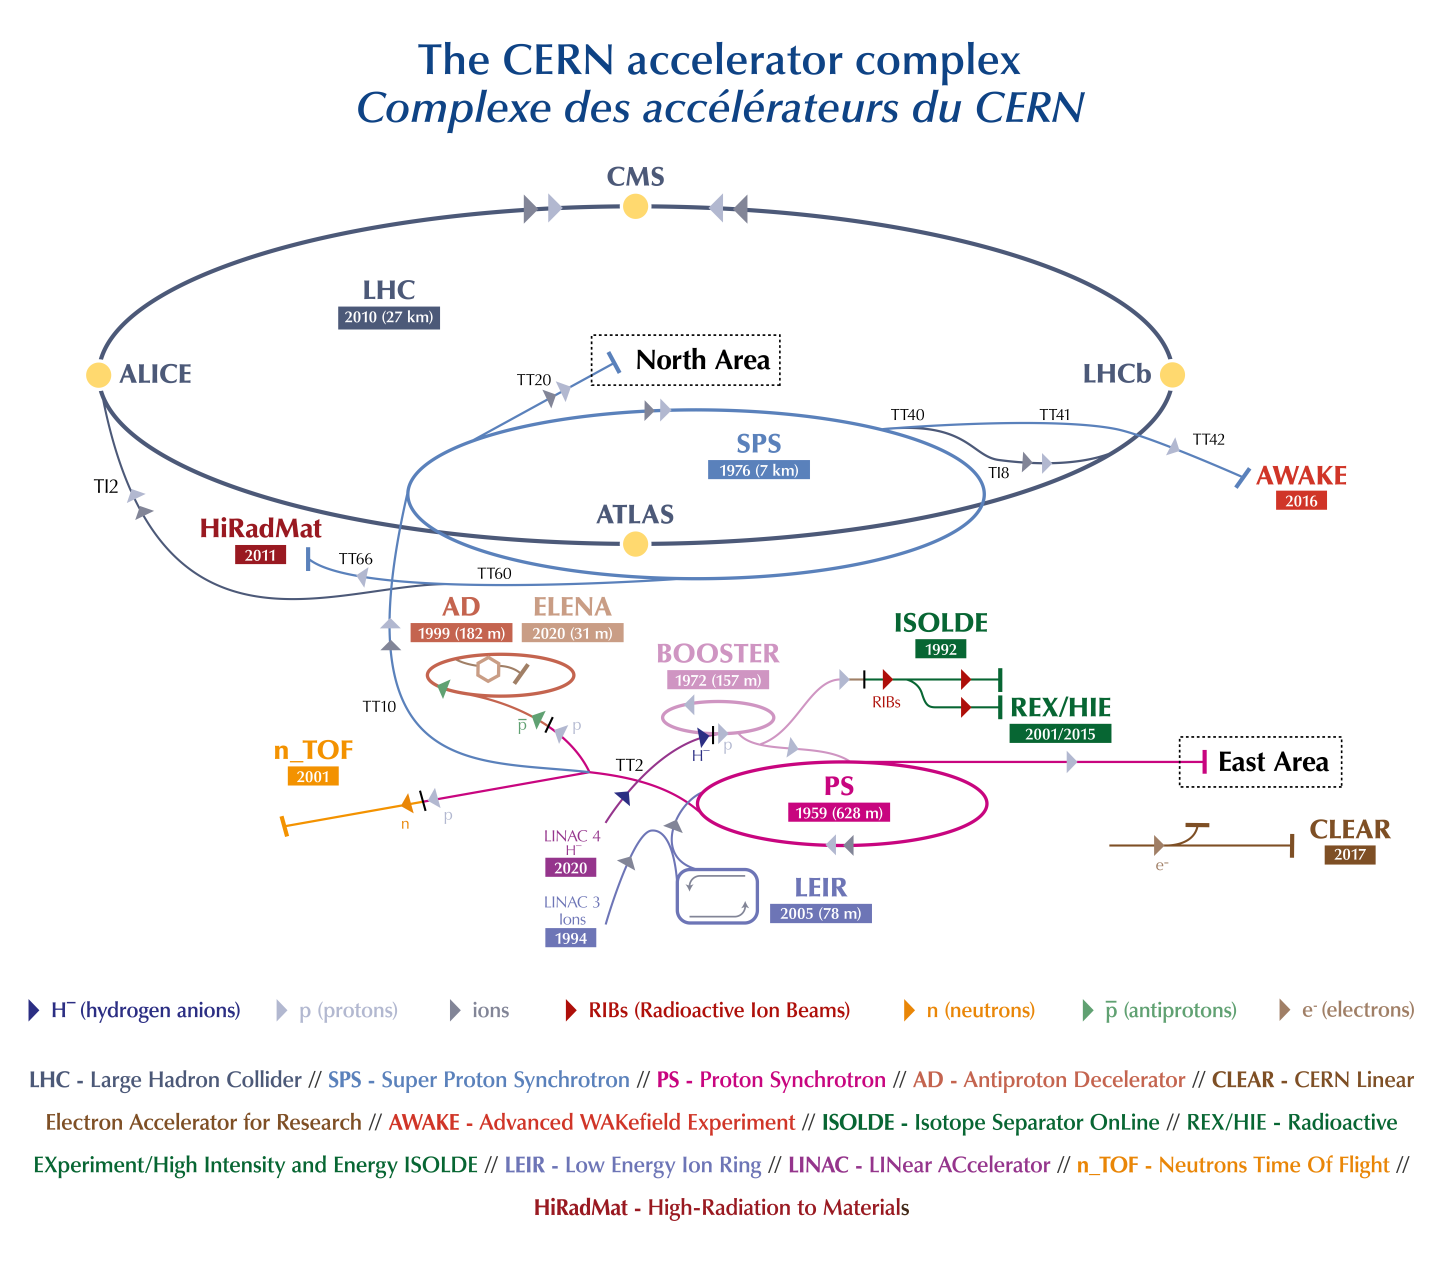
\includegraphics[width=0.65\textwidth]{images/LHC_complex.png}
  \caption{...}
  \label{LHC_complex}
  % https://cds.cern.ch/record/2684277?ln=es
\end{figure}

El último de los aceleradores es el LHC, donde los protones circulan en direcciones opuestas por cavidades de ultra alto vacío a una presión de $10^{-10}$ torr. El mismo cuenta con $1232$ dipolos magnéticos superconductores de 15 m de largo enfriados a $1.9$ K mediante helio superfluido, que generan un campo magnético de $8.4$ T y permite mantener en su órbita circular a los protones. Los dipolos están equipados con sextupolos, octupolos y decapolos, que permiten corregir las pequeñas imperfecciones del campo magnético en las extremidades de los dipolos. Para aumentar la probabilidad de colisión, existe un sistema de focalización de los haces en las proximidades de los detectores, que estrecha el camino que recorren los protones. El mismo consiste de $392$ cuadrupolos magnéticos que generan campos magnéticos de $6.8$ T. 

Los protones son acelerados mediante cavidades de radiofrecuencia que generan un voltaje longitudinal a una frecuencia específica. En esa frecuencia los protones sincronizados con la energía deseada no van sufrir aceleración alguna, mientras que aquellos descincornizados van a ser acelerados o desacelerados hasta obtener la energía deseada. De esta forma el haz de protones se divide en paquetes discretos denominados \textit{bunches}, cada uno conteniendo del orden de 10$^{11}$ protones. El número de \textit{bunches} totales posibles en un haz con un espaciado de 25 ns es de 3564 \footnote{Se obtiene al dividir la frecuencia de las cavidades, 400 MHz, por la frecuencia de revolución, 11 kHz, y considerando que sólo 1 de cada 10 \textit{bunches} es llenado para lograr el espaciado deseado}. Considerando los tiempos que se necesitan para en la inyección y descarte del haz, junto con los tiempos que necesita cada detector para procesar la información, no todos los \textit{bunches} son llenados, sino que se dejan `espacios' definidos por diferentes esquemas, dejando así el número efectivo de \textit{bunches} llenos a 2808.

Los aceleradores pueden ser caracterizados no solo por su energía de centro de masa sino también por su luminosidad instantánea ($\mathcal{L}$), que mide el número de colisiones que ocurren en un período de tiempo y se define como: 

\begin{equation}
\mathcal{L}=f_{\text{rev}}n_{b}\frac{N_{1}N_{2}}{A}
\end{equation}

\noindent
donde $f_{\text{rev}}$ es la frecuencia de revolución ($\sim$11 kHz), $n_{b}$ es el número de \textit{bunches} por haz, $N_{i}$ es el número de partículas en cada \textit{bunch} y \textit{A} es la sección efectiva del haz, que puede expresarse en término de los parámetros del acelerador como:

\begin{equation}
A=\frac{4 \pi \epsilon_{n}\beta^{*}}{\gamma F}
\end{equation} 

\noindent
donde $\epsilon_{n}$ es la emitancia transversal normalizada (la dispersión transversal media de las partículas del  haz en el espacio de coordenadas e impulsos), $\beta^{*}$ es la función de amplitud en el punto de interacción, relacionada al poder de focalización de los cuadrupolos), $\gamma$ es el factor relativista de Lorentz y \textit{F} es un factor de reducción geométrico, debido al ángulo de cruce de los haces en el punto de interacción.

El número total de eventos esperados para un dado proceso con una sección eficaz $\sigma$, se obtiene como:

\begin{equation}
N=\sigma \int \mathcal{L} dt
\end{equation}	

\noindent
donde al factor integral se lo conoce como luminosidad integrada.

El LHC comenzó a funcionar en 2010 en lo que se denominó \textit{Run 1}, a una energía de de centro de masa de 7 TeV y logrando recolectar <<<lumi>>. En el 2013 finaliza la toma de datos y comienza el \textit{Long shutdown 1}, período que se utilizó para realizar distintas actualizaciones preparándose para la siguiente toma de datos. En el 2015 comenzó el \textit{Run 2} que operaba a una energía de de centro de masa de 13 TeV y logró recolectar <<<lumi>>, finalizando en el 2018 dando lugar al \textit{Long shutdown 2}. Este último estaba previsto con una duración de dos años, pero dada la situación epidemiológica de COVID-19 el mismo se terminó extendiendo hasta (???). Los planes a futuro del LHC preveen un tercer \textit{run} a 14 TeV, y luego ingresar en un nuevo período de inactividad para realizar las mejoras necesarias para el \textit{High Luminosity LHC}.





\section{El detector ATLAS}

ATLAS (\textit{\textbf{A} \textbf{T}oroidal \textbf{L}HC \textbf{A}pparatu\textbf{S}})  \cite{PERF-2007-01} es uno de los experimentos multipropósito del LHC, diseñado para estudiar las colisiones protón-protón a altas energías provistas por el LHC.

El mismo tiene una simetría aproximadamente cilíndrica y está compuesto de distintos subdetectores, que cumplen diversas funciones en la identificación de las partículas producidas durante las colisiones. En la zona más próxima al haz se encuentra detector interno de trazas (ID) cuyo objetivo principal es reconstruir la trayectoria de las partículas cargadas. Está compuesto del Insertable B-Layer (IBL), un detector de píxeles, un detector de bandas de silicio (SCT) y un detector de radiación de transición (TRT). A su vez, envolviendo al ID, se encuentra un solenoide superconductor que genera un campo magnético de $2$ T, el cual curva la trayectoria de las partículas cargadas permitiendo así medir su impulso.

A continuación se ubica el sistema de calorímetros compuesto por el calorímetro electromagnético (ECAL) que mide principalmente la energía depositada por fotones y electrones, y el calorímetro hadrónico (HCAL) para medir la energía de los jets y hadrones.

En la parte más externa, se encuentra el espectrómetro de muones (MS) diseñado para detectar la producción de muones y además medir su momento. Este último es el que le da a ATLAS su tamaño característico de $45$ m de largo y $25$ m de alto. Intercalado con el MS se encuentra un sistema de imanes toroidales, que generan un campo magnético de $4$ T para curvar la trayectoria de los muones hacia el final del detector.

El detector ATLAS se divide geométricamente en dos regiones, la parte central denominada \textit{barrel} y la región extrema \textit{endcap}. En la región \textit{barrel} los detectores se ubican en forma de cilindros concéntricos alrededor del eje del haz, mientras en la región \textit{endcap} se disponen como discos perpendiculares a la dirección del haz. 

La Figura \tosolve{agregar figura} detalla todas las componentes que integran al detector ATLAS y son descriptas en detalle a en las siguientes secciones.

\section{Sistema de coordenadas}

El sistema de coordenadas de ATLAS corresponde a un sistema cartesiano, cuyo origen coincide con el punto de interacción nominal ubicado en el centro del detector. El eje \textit{z} está orientado con hacia la dirección del haz, el eje \textit{x} se define desde el punto de interacción hacia el centro del anillo del LHC, y el eje \textit{y} se define apuntando hacia la superficie terrestre.

Es conveniente además definir un sistema de coordenadas cilíndricas donde el radio \textit{R} representa la distancia perpendicular al haz, el ángulo azimutal $\phi$ es medido alrededor del eje del haz, y el ángulo polar $\theta$ se mide con respecto al eje del haz perpendicular al eje \textit{x}. 

Una variable utilizada en física experimental de altas energías es la rapidez:

\begin{equation}
y=\frac{1}{2}\ln\left( \frac{E+p_{z}}{E-p_{z}}\right)
\end{equation}

\noindent
donde \textit{E} es la energía total de la partícula y $p_{z}$ es la componente en la dirección del haz de su impulso\footnote{Esta definición es un caso particular de la rapidez utilizada en relatividad especial, cuando se realiza una transformación en la dirección del haz del sistema de la boratorio a un sistema donde la partícula solo se mueve perpendicular al haz.}. En el límite de altas energías, en donde la masa de la partícula es despreciable frente a su momento, es posible aproximarla a la llamada pseudorapidez $\eta$:

\begin{equation}
\eta =-\ln \tan\left( \frac{\theta}{2} \right)
\end{equation}

\noindent
estando completamente relacionada con el ángulo $\theta$. La razón detrás de esta transformación de coordenadas se debe a que la multiplicidad de partículas producidas es aproximadamente constante como función de $\eta$, y que la diferencia de pseudorapidez entre dos partículas es invariante frente a transformaciones de Lorentz a lo largo de la dirección del haz. 

% dR y editar parrafo que sigue!

En el caso de colisiones hadrónicas, la fracción del impulso del protón adquirida por cada uno de las partones interactuantes es desconocida. Parte de este impulso es transferido en la interacción dura, mientras cierta fracción remanente escapa el detector a lo largo del haz. De esta forma, no es posible reconstruir el movimiento longitudinal del centro de masa en la interacción, y aplicar leyes de conservación sobre la cinemática de cada evento. Sin embargo, dado que los protones inciden a lo largo de la dirección del haz, y asumiendo que el momento de los partones en la dirección transversa al haz es nulo, el impulso total transverso se conserva durante la colisión. Por este motivo, es común utilizar solo las componentes transversales en la descripción de la cinemática del evento, definidas en términos de la pseudorapidez, como por ejemplo el momento transverso:

\begin{equation}
p_{T}=p\sin\theta=\frac{p}{\cosh{\eta}}
\end{equation}

\noindent
donde \textit{p} es el momento de la partícula. De esta forma es posible describir la cinemática de cada partícula en términos de ($\pt$, $\eta$, $\phi$)

\section{Sistema de imanes}

El detector ATLAS posee un poderoso sistema de imanes \cite{magnet} utilizado para curvar la trayectoria de las partículas cargadas, pudiendo así medir tanto su impulso de forma precisa como también su carga. El mismo consta de dos tipos de imanes superconductores, uno en forma solenoidal y otros tres forma toroidal, enfriados a una temperatura de 4.5 K para poder producir los fuertes campos magnéticos.

El solenoide rodea al detector interno, y tiene un tamaño de 5.6 m de largo y 2.56 m de diámetro \commentNotaIV, y con un espesor de apenas 4.5 cm. El mismo produce un campo magnético de 2 T en la dirección del haz, por lo que las partículas cargadas son curvadas en la dirección de $\phi$ \tosolve{revisar}. Para minimizar la interacción de las partículas que lo atraviesan y ahorrar la mayor cantidad de material posible, el solenoide comparte la cámara de vacío del calorímetro de LAr (\tosolve{sección...})

Los toroides de ATLAS se componen de ocho bobinas, que generan campos de hasta 4 T \tosolve{mirar bien estos números} en la dirección $\phi$, por lo que las partículas que lo atraviesan (muones) so curvadas en la dirección $\eta$. El más grande de ellos mide 25.3 m de largo y 20.1 m de diámetro, y se ubica en la parte más externa del detector \textit{barrel} intercalado con el Espectrómetro de Muones (\tosolve{seccion...}). Los otros dos restantes se encuentran en la región \textit{endcap}, por fuera de los calorímetros, y miden 5.0 m de largo y 10.7 m de diámetro. 



\section{Los subdetectores de ATLAS}

\subsection{Detector interno}

El detector interno es el más próximo al haz y su función principal es la reconstrucción de las trazas de las partículas cargadas, que a su vez sirve para medir la dirección, momento y carga de la misma, y la reconstrucción de los vértices primarios. Para ello combina detectores de muy alta resolución cerca del haz, junto con detectores continuos de trazas en la zona más alejada. El principio básico de funcionamiento consiste en utilizar su alta granularidad, para mapear las señales que dejan las partículas al atravesar cada celda, en coordenadas espaciales. El conjunto de esas señales son reconstruidas como trazas mediante algoritmos especializados. El detector interno contenido dentro del solenoide superconductor y mide 6.2 m de largo y 2.1 m de diámetro. 

\subsubsection{Detector de píxeles}

El detector de píxeles fue construido para medir la posición de las trazas de partículas cargadas con la más alta precisión posible y es de vital importancia para la reconstrucción de los vértices primarios y secundarios. En la región \textit{barrel} el detector se compone de tres capas cilíndricas, mientras que la \textit{endcap} de tres discos. La capa más interna, denominada \textit{B-Layer}, se encuentra a $50.5$ mm del punto de interacción. El principio de detección para partículas cargadas es la medida de la deposición de la carga inducida en una capa de silicio por ionización. El sistema contiene un total de $80$ millones de sensores, cada uno con una resolución de $10\:\mu$m ($R-\phi$) y $115\:\mu$m ($z$).

Luego del Run 1 la luminosidad del LHC aumentó notablemente, lo que podía significar un daño por radiación en los detectores internos. En vez de reemplazar las partes del detector de píxeles que podían ser dañadas, se decidió colocar una capa adicional entre el detector de píxeles y la tubería donde circulan los protones denominado \textit{Insertable B-Layer} \cite{ATLAS-TDR-2010-19}. El objetivo del mismo es mejorar la eficiencia en la identificación de trazas, vértices, y en la identificación de \textit{bottom} quarks, que decaen típicamente fuera del radio del IBL.

El IBL está compuesto por $8$ millones de chips de rápida lectura y con sensores de silicio, que detectan el paso de partículas cargadas mediante la deposición de carga inducida. El tamaño de los píxeles es de $50\times250\:\mu$m$^{2}$, con una resolución de $8\:\mu$m ($R-\phi$) y $40\:\mu$m ($z$). La distancia entre el IBL y la tubería es de $0.2$ mm, y entre el tubo y el detector de píxeles es de $1.9$ mm. 

% the modules in the barrels are slightly overlapping and rotated to provide full azimuthal coverage

\subsubsection{Detector Semiconductor de Trazas (SCT)}

Se encuentra por fuera del detector de píxeles y está diseñado para medir las trazas con alta precisión en la zona intermedia del detector. A diferencia del detector de píxeles, estos sensores de silicio están segmentados en micro bandas, dado que es más baja multiplicidad de partículas es posible reducir la resolución al costo de aumentar el área de cobertura. La resolución de $17\:\mu$m ($R-\phi$) y $580\:\mu$m ($z$). En la región \textit{barrel} los módulos de SCT están dispuestos en 4 capas concéntricas, mientras que en la región \textit{endcap} consiste en 9 discos transversales al eje del haz.

% the modules in the barrels are slightly overlapping and rotated to provide full azimuthal coverage

\subsubsection{Detector de Radiación de Transición (TRT)}

Es el detector más externo del ID y está diseñado, no solo para detectar partículas cargadas, sino también para distinguir entre partículas pesadas y livianas. El TRT se compone de tubos detectores de $4$ mm de diámetro, con un gas que ioniza al ser atravesado por partículas cargadas. Los electrones producidos son colectados por una ánodo, y el tiempo de deriva es una medida de la distancia a la traza del mismo. Además, los tubos están rodeados de fibras de polipropileno con un índice de refracción diferente, por lo que las partículas que atraviesan el detector emiten radiación con una intensidad proporcional a $\gamma=E/m$, permitiendo al TRT  distinguir partículas cargadas pesadas ($\pi^{\pm}$) de aquellas más livianas ($e^{\pm}$). La región \textit{barrel} contiene $50000$ tubos paralelos al eje del haz y la región \textit{endcap} $320000$ tubos orientados radialmente. Su resolución es de $0.17$ mm.

\subsection{Calorímetros}

El sistema de calorímetros de ATLAS está diseñado para medir la energía y la posición de las partículas, mediante la absorción de la energía depositada por las cascadas de partículas secundarias que estas generan en el material del mismo. Además, permite discriminar electrones y fotones de jets, detectar aquellas partículas neutras que no dejaron trazas en el ID y realizar la selección \textit{online} de eventos potencialmente interesantes (Ver Sistema de \textit{trigger}). Gracias a su amplia cobertura y a que absorbe la energía de prácticamente todas las partículas producidas (salvo muones) es de gran utilidad para poder medir el desbalance de energía transversa, magnitud discriminatoria utilizada en la mayoría de análisis fuera del SM.

Está compuesto de un calorímetro electromagnético (ECAL) dedicado principalmente a la medida de las deposiciones de partículas como fotones y electrones (partículas interactuantes principalmente vía interacción EM), y otro hadrónico (HCAL) dedicado a las cascadas de partículas producto de la hadronización de los quarks o gluones (\textit{jets}) (partículas interactuantes principalmente vía interacción fuerte).

\subsubsection{Calorímetro electromagnético (ECAL)}

El ECAL en un calorímetro de muestreo (inhomogéneo) no compensado, que utiliza Plomo como material absorbente y LAr como material absorbente. Consiste en varias placas de Plomo dispuestas en forma de acordeón que se colocan de forma alterna inmersas en LAr. Las partículas incidentes interactúan con el Plomo creando una lluvia de partículas cargadas y neutras. Las partículas cargadas ionizan el medio activo, donde los electrones liberados son colectados en un electrodo central de kaptón/Cu hacia donde derivan por acción del campo eléctrico aplicado. La señal total en el medio activo es así proporcional a la energía total real de la partícula incidente. La ventaja de este método es la detalla reconstrucción de la forma de la cascada, al costo de no poder reconstruir la totalidad de la energía de la cascada debido al espacio que existe entre placa y placa.


El ECAL está dividido en dos mitades dentro de la
región \textit{barrel} ($\eta < 1.475$) y en dos componentes (una a cada
lado) en la región \textit{endcap} ($1.375 < |\eta| < 3.2$) En la región de transición entre el \textit{barrel} y el \textit{endcap} se encuentra una zona no instrumentada, por donde se conecta el detector. Esta región, denominada \textit{crack}, está comprendida entre $1.37 < |\eta| < 1.52$. Es por este motivo que la mayoría de los análisis se requiere que los candidatos a fotones/electrones estén fuera de la región \textit{crack}.

En la región diseñada para medidas de precisión ($\eta < 2.5$, excluyendo el \textit{crack}),
el ECAL está segmentado en tres capas longitudinales. La primera capa consiste de
bandas con fina granularidad (en la dirección de $\eta$), para discriminar entre fotones
aislados y pares de fotones espacialmente cercanos provenientes del decaimiento
$\pi^0\to\gamma\gamma$. Para los electrones y fotones con alta energía transversa, la mayoría
de la energía se colecta en la segunda capa, que tiene una granularidad lateral de
$0.025 \times 0.025$ en $(\eta, \phi)$. La tercer capa se encarga de la energía depositada en las
colas de la lluvia.
El espesor del ECAL es mayor a 22 longitudes de radiación ($X_0$) en la región
barrel, y mayor a 24 $X_0$ en los endcap, donde una longitud de radiación se define
como la distancia promedio sobre la cual la energía de un electrón se reduce a $1/e$
de su energía inicial. Para el caso de los fotones, una reducción similar se obtiene a
9/7 de $X_0$ . Por tanto, toda la energía electromagnética es absorbida en el ECAL y
sólo parte de la componente hadrónica llega al HCAL.

\subsubsection{Calorímetro hadrónico (HCAL)}

El HCAL es un conjunto de calorímetros que rodean al ECAL, extendiendo la aceptancia del calorímetro de ATLAS hasta cubrir prácticamente la totalidad de ángulo sólido del punto de colisión.

El primero de los calorímetros se denomina \textit{Tile Calorimeter}, es un calorímetro de muestreo que utiliza acero como material absorbente y tejas centelladoras plásticas como material activo, se encuentra en la región \textit{barrel} y está dividido en dos partes que tienen una cobertura de $|\eta|<1.0$ y $0.8<|\eta|<1.7$ respectivamente. 
% Los centelladores, dispuesto en un arreglo
% periódico, se conectan a una fibra óptica que trasporta la luz producida por el paso
% de partículas, hacia un tubo fotomultiplicador. Este arreglo se extiende, en R, de los
% 2.28 a los 4.25 m. 
En la región \textit{endcap} se encuentra un calorímetro hadrónico de muestreo (HEC) con placas de cobre como absorbente y argón líquido como material activo, que consiste en dos ruedas, una atrás de la otra con las placas planas de Cu dispuestas perpendicularmente al eje del haz, conn un radio de 2.3 m. Finalmente se encuentra el Forward Calorimeter (FCAL), un calorímetro de muestreo que extiende la cobertura del sistema a $|\eta|<4.9$, coaxial
al eje del haz y ubicado a 4.7 m a cada lado del punto de interacción. El material
principal de los módulos es argón líquido (con cobre o tungsteno), y si bien no se
utiliza para mediciones de precisión, provee información para el cómputo de la ener-
gía transversa faltante y la reconstrucción de jets en regiones muy cercanas al eje
del haz.



Por su parte, el HCAL tiene un espesor mayor a 7.7 longitudes de interacción
hadrónica ($\lambda$) en la región barrel (9.7$\lambda$ en total si se cuenta el ECAL). De manera
análoga a la longitud de radiación mencionada para el ECAL, una longitud de
interacción hadrónica se define como la distancia promedio sobre la cual la energía
de un hadrón se reduce a $1/e$ de su energía inicial. De esta forma, toda la energía
con la que llegan los hadrones al HCAL, queda allí depositada.

\subsection{Espectrómetro de muones}

El espectrómetro de muones (MS) se encuentra situado en la parte más externa del detector ATLAS. Esto se debe a que los muones de alto $p_{T}$ generados en el punto de interacción tienen un altísimo poder de penetración y son poco interactuantes, siendo las únicas partículas detectables capaces de llegar a este detector. El mismo se encuentra intercalado con el sistema de imanes toroidales, y está diseñado para obtener mediciones de alta precisión de la posición e impulso de los muones, y para una rápida identificación para el sistema de \textit{trigger}. Este es el subdetector más grande y el que le da a ATLAS su tamaño característico. 

El MS se compone de diferentes tipos de cámaras de detección de muones (ver Figura \ref{muon}). Las \textit{Monitored Drift Tubes} (MDTs) son responsables de la mayoría de las medidas de precisión y cubren el rango de $|\eta|<2.7$. Funcionan de forma similar al TRT, con tubos llenos de un gas que ioniza y un ánodo central que recoge los electrones producidos, y el tiempo de deriva se asocia con la distancia a la traza. En la región \textit{endcap} se encuentran las \textit{Cathode Strip Chambers} (CSCs) que poseen alta resolución espacio-temporal y una cobertura $|\eta|>2.0$. Estas cámaras funcionan midiendo la carga depositada en un ánodo, producto de la cascada de electrones creados cerca del mismo. Las \textit{Resistive Plate Chamber} (RPCs) proveen una estimación rápida del momento de los muones al primer nivel del \textit{trigger} con una cobertura de $|\eta|<1.05$. Las RPCs miden la descarga ocasionada entre dos placas resistivas paralelas sometidas a una alta diferencia de potencial, tras la ionización del volumen de gas interno causada por el paso de muones energéticos. Finalmente se encuentra en la región \textit{endcap} las \textit{Thin Gap Chambers} (TGCs), similares en funcionamiento a las CSCs. Proveen también información al sistema de \textit{trigger} en esta región y tienen una cobertura de $|\eta|<2.4$.

\section{Sistema de \textit{trigger}}

\section{Modelo computacional y distribución de datos}
